\begin{frame}{Gravsøgende jagthunde}

\vspace{1em}

\begin{columns}[c] % c = center vertically

\column{0.05\textwidth} % Venstre margin

\column{0.7\textwidth} % Midten: Bullets

\small

\raggedright

\begin{itemize}

\itemsep0.6em % Justér afstand mellem bullets

\item Hundens opgave er at \textbf{lokalisere og drive vildtet ud af hulen} (gravjagt).
\item Anvendes primært til jagt på \textbf{ræv} i deres huler (grave).
\item Hundene skal have et \textbf{hårdt og modigt sind} og være fysisk rustede til trange miljøer.
\item Gravjagten er en \textbf{særlig jagtform} og er reguleret af Miljøstyrelsen.
\item \textbf{Racer}: Fox Terrier, Jack Russell Terrier, Tysk Jagtterrier, Gravhunde.

\end{itemize}

\column{0.25\textwidth} % Højre: Ikon

\centering

\vspace{0pt}

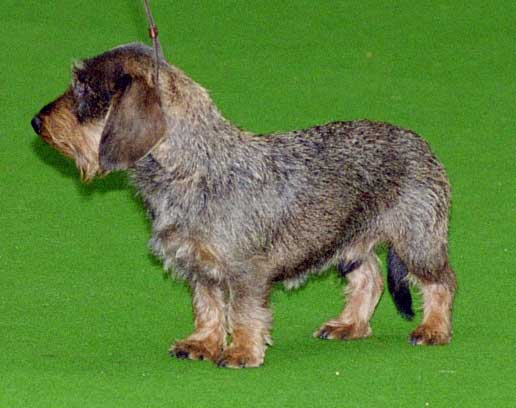
\includegraphics[width=0.9\linewidth]{Billeder/Jagthunde/gravsoegende/gravhund.jpg} % Ikon af gravsøgende hund/gravhund

\end{columns}

\end{frame}